%%
%%
%% beamerthemethuas-doc.tex
%%
%% Definitions for the beamer layout for
%%
%% The Hague University of Applied Sciences (THUAS)
%%
%% (c)2021 J. op den Brouw  <J.E.J.opdenBrouw@hhs.nl>
%%
%%
%% This work may be distributed and/or modified under the
%% conditions of the LaTeX Project Public License, either version 1.3
%% of this license or (at your option) any later version.
%% The latest version of this license is in
%%   http://www.latex-project.org/lppl.txt
%% and version 1.3 or later is part of all distributions of LaTeX
%% version 2005/12/01 or later.
%%
%% This work has the LPPL maintenance status `maintained'.
%% 
%% The Current Maintainer of this work is J.E.J. op den Brouw
%%
%% This work consists of the files
%%   beamerthemethuas.sty
%%   beamerinnerthemethuas.sty
%%   beamerouterthemethuas.sty
%%   beamercolorthemethuas.sty
%%   beamerthemethuas-doc.tex
%%   beamerthemethuasfront.pdf
%%   beamerthemethuaslogo.pdf
%%   beamerthemethuaslogo-en.pdf
%%
%% and the derived file beamerthemethuas-doc.pdf
%%

%% Use ``dutch'' as class option
\documentclass[fleqn,aspectratio=169,dutch]{beamer}

%% Babel is needed for correct translations
%% It needs the ``dutch'' option
\usepackage[dutch]{babel}

%% Show frames, for testing
%\usepackage{showframe}

%% The THUAS beamer style, loads the correct fonts
\usetheme[nav]{thuas}

%% PGFplots
\usepackage{pgfplots}
\usepgfplotslibrary{fillbetween}
\usepgfplotslibrary{patchplots}
\pgfplotsset{compat=1.3}

%% Nice listings
\usepackage{listings}
\lstset{
    language=C,
    basicstyle=\ttfamily\small,
    xleftmargin=1em,
}

%% Nice tables, no vertical bars!
\usepackage{booktabs}

%% Typeset quantities in math mode
%\usepackage{siunitx}

%% Set up credentials
\title{THUAS Beamer Slides}
\subtitle{De THUAS layout maar nu met Beamer}
\author{Jesse op den Brouw}
\date{\today}

%%
%%
%%
\begin{document}

%% Title page
\maketitle


\begin{frame}[fragile]{THUAS Beamer Slides}
\begin{itemize}
\item Dit is de onofficiële realisatie van slides met het THUAS-thema
\item Eerst gebruik je de beamer-class: \lstinline|\documentclass{beamer}|
\item Daarna laadt je de theme met: \lstinline|\usetheme[|\emph{\small opties}\lstinline|]{thuas}|
\item Het werkt met \LaTeX, Xe\LaTeX en Lua\LaTeX
\item Werkt met Nederlands en Engels
\item De titelpagina is niet conform de regels, maar komt in de buurt
\end{itemize}
\end{frame}


\begin{frame}[fragile]{THUAS Beamer Slides}
\begin{itemize}
\item De officiële realisatie is met aspect ratio 16:9, dus:
\begin{itemize}
\item Gebruik \lstinline|\documentclass[aspectratio=169]{beamer}|
\end{itemize}
\item Maar sommige beamers werken nog met 4:3, dus:
\begin{itemize}
\item Gebruik \lstinline|\documentclass[aspectratio=43]{beamer}|
\end{itemize}
\item Er zijn nog andere formaten maar die worden niet ondersteund
\item Er zijn verschillen in de titelpagina tussen 16:9 en 4:3
\begin{itemize}
\item Dat komt o.a.\@ door het plaatsen van het plaatje op de titelpagina
\end{itemize}
\item Er zijn verschillen tussen Xe-, Lua- en pdf\LaTeX
\begin{itemize}
\item Dat komt o.a.\@ door de vorm en de grootte van de gebruikte fonts
\end{itemize}
\end{itemize}
\end{frame}


\begin{frame}[fragile]{THUAS Beamer Slides}
\begin{itemize}
\item Nederlands en Engels worden ondersteund.
\item Nederlands is de standaard taal.
\begin{itemize}
\item Gebruik \lstinline|\usetheme[dutch]{thuas}|.
\item Op de titelpagina en in de slides wordt dan het Nederlandse logo gebruikt.
\end{itemize}
\item Engels kan ook gebruikt worden.
\begin{itemize}
\item Gebruik \lstinline|\usetheme[english]{thuas}|.
\item Op de titelpagina en in de slides wordt dan het Engelse logo gebruikt.
\end{itemize}
\end{itemize}
\end{frame}

\begin{frame}[fragile]{THUAS Beamer Slides}
\begin{itemize}
\item Standaard wordt 11pt fontgrootte gebruikt.
\item Dit kan je met een class optie aanpassen, bijvoorbeeld \lstinline|\documentclass[10pt]{beamer}|
\item Er zijn verschillende fontgroottes: 
\begin{itemize}
\item 8pt, 9pt, 10pt, 11pt (default), 12pt, 14pt, 17pt en 20pt.
\item 10pt en 11pt zijn de meest gangbare varianten.
\end{itemize}
\end{itemize}
\end{frame}

\begin{frame}[fragile]{THUAS Beamer Slides}
Om correct gebruik te maken van het Nederlands, gebruik
\begin{lstlisting}
\documentclass[dutch]{beamer}
\end{lstlisting}
en
\begin{lstlisting}
\usepackage[dutch]{babel}
\end{lstlisting}
Dan worden environments als \lstinline|theorem| en \lstinline|proof| van de correcte namen voorzien

\alert{TODO}: automatisch laden van \lstinline|babel| met \lstinline|dutch| of \lstinline|english|
\end{frame}


\begin{frame}[fragile]{THUAS Beamer Slides}
Xe\LaTeX{} en Lua\LaTeX:
\begin{itemize}
\item Het standaard font is Arial voor lopende tekst en Arial Black voor titels
\item Het standaard font voor formules is Cambria Math
\item Het standaard font voor programmacode is Consolas
\item Deze fonts worden automatisch geladen
\item Wil je andere fonts gebruiken, gebruik dan \lstinline|\usetheme[vanilla]{thuas}|
\end{itemize}
\end{frame}


\begin{frame}[fragile]{THUAS Beamer Slides}
pdf\LaTeX{}:
\begin{itemize}
\item Het standaard font is Helvet voor lopende tekst en Helvet/bold voor titels
\item Het standaard font voor formules is Libertinus Math
\item Het standaard font voor programmacode is Nimbus Mono
\item Deze fonts worden automatisch geladen
\item Wil je andere fonts gebruiken, gebruik dan \lstinline|\usetheme[vanilla]{thuas}|
\end{itemize}
\end{frame}


\begin{frame}[fragile]{THUAS Beamer Slides}
\begin{itemize}
\item Subtitel op titelpagina wordt \emph{niet} weergegeven
\begin{itemize}
\item Deze subtitel wordt gewoon genegeerd
\end{itemize}
\item Subtitels op frames worden \emph{niet} weergegeven
\begin{itemize}
\item Deze subtitels worden gewoon genegeerd
\end{itemize}
\item De inhoud van een slide wordt \emph{niet} gecentreerd
\begin{itemize}
\item De huisstijl is zo
\item Wil je toch gecentreerde slides, gebruik dan \lstinline|\usetheme[c]{thuas}|
\end{itemize}
\item Maak een allerlaatste slide met \lstinline|\beamerthemethuasbackframe|
\end{itemize}
\end{frame}


\begin{frame}[fragile]{THUAS Beamer Slides}
\begin{itemize}
\item Navigatie-buttons komen rechts boven
\begin{itemize}
\item Gebruik \lstinline|\usetheme[nav]{thuas}|
\end{itemize}
\item Als je handouts wilt maken, gebruik dan de \lstinline|handout| optie
\begin{itemize}
\item Gebruik \lstinline|\documentclass[handout]{beamer}|
\item Dit is een optie voor \lstinline|beamer|
\end{itemize}
\item Als je het totaal aantal slides naast het slidenummer wil gebruiken
\begin{itemize}
\item Gebruik \lstinline|\usetheme[numpages]{thuas}|
\item Werkt niet lekker met voetnoten
\end{itemize}
\end{itemize}
\end{frame}


\beamerthemethuaslogofalse

\begin{frame}[fragile]{THUAS Beamer Slides}
\begin{itemize}
\item Standaard wordt het logo rechtsonder weergegeven, behalve bij de titelpagina
\item Het logo kan je uitzetten met \lstinline|\beamerthemethuaslogofalse|
\item Het logo blijft dan uit
\item Het logo kan je aanzetten met \lstinline|\beamerthemethuaslogotrue|
\item Het logo blijft dan aan
\item Op deze slide is het logo uit
\end{itemize}
\end{frame}

\beamerthemethuaslogotrue


\begin{frame}{Formules kunnen ook}
\begin{itemize}
\item De formules zijn (met behulp van een \lstinline|align*| environment):
\begin{align*}
\left|F(x)\right|^b_a &= \int_a^b x^2 + 2x + 1 \, \mathrm{d} x \\
\zeta (s) &= \sum_{n=1}^\infty \dfrac{1}{n^{\;\!s}} \\
M&\approx\frac{\pi}{4}\left(\frac{2d}{\lambda_o}\right)^2\left(\mathrm{NA}\right)^2
\end{align*}
\end{itemize}
\end{frame}


\begin{frame}{Formules kunnen ook}
Nu zonder itemize (met behulp van \lstinline|equation*| en \lstinline|multiline*|)
\begin{equation*}
\tan \alpha = \dfrac{\sin \alpha}{\cos \alpha} \qquad \tan x = \sin x \, / \cos x
\end{equation*}
\begin{multline*}  
K=\displaystyle{\frac{1}{2}m_1 L_1^2 \dot{\theta_1}^2+\frac{1}{2} m_2[L_1^2 \dot{\theta_1}^2+L_2^2 \dot{\theta_2}^2+2 L_1 L_2 \dot{\theta_1}\dot{\theta_2}\cos(\theta_1-\theta_2)]} \\
 \displaystyle{+\frac{1}{2}m_3[L_1^2 \dot{\theta_1}^2+L_2^2 \dot{\theta_2}^2+L_3^2+ \dot{\theta_3}^2+2 L_1 L_2 \dot{\theta_1}\dot{\theta_2}\cos(\theta_1-\theta_2)}
\end{multline*}
\begin{equation*}
\mathrm{e}^{\, \mathrm{j}\alpha} = \cos \alpha + \mathrm{j} \sin \alpha
\end{equation*}
\end{frame}


\begin{frame}{Voorbeeld met een itemize}

Voorbeeld met een \texttt{itemize} en gaat tot drie niveaus diep.
\begin{itemize}
\item item
\begin{itemize}
\item sub item
\begin{itemize}
\item sub sub item
\end{itemize}
\end{itemize}
\item item
\end{itemize}
Meer niveaus zijn in \lstinline|beamer| niet mogelijk.
\end{frame}


\begin{frame}{Voorbeeld met een enumerate}
Voorbeeld met een \texttt{enumerate} en gaat tot drie niveaus diep.
\begin{enumerate}
\item een
\item twee
\begin{enumerate}
\item een
\item twee
\begin{enumerate}
\item een
\item twee
\end{enumerate}
\end{enumerate}
\item drie
\end{enumerate}
Meer niveaus zijn in \lstinline|beamer| niet mogelijk.
\end{frame}


\begin{frame}{Voorbeeld van een description}
De label wordt vet en rechts uitgelijnd afgedrukt

De label kan ongeveer 9 karakters bevatten

Daarna wordt er ingesprongen
\begin{description}
\item[123456789] Dit is een hele lange tekst en ik denk dat deze zin over twee regels verspreid zal zijn
\item[label] description
\item[deze label is te groot] description
\end{description}
\end{frame}


%% A frame with a listing NEEDS fragile
\begin{frame}[fragile]{Een frame met code}
Een frame met daarin code met \texttt{lstlistings} moet getypeerd worden met \texttt{fragile}, anders werkt het niet

\begin{lstlisting}
\begin{frame}[fragile]{Titel}
\end{lstlisting}

Voorbeeld:

\begin{lstlisting}
#include <stdio.h>

int main(void) {
    printf("THUAS Beamer Slides!\n");
}
\end{lstlisting}

Niet getest met \lstinline|minted|
\end{frame}


\begin{frame}[fragile]{Voetnoot en plaatje}
Een voetnoot\footnote{Dit is een voetnoot}. Gebruik liever geen voetnoot.

Een plaatje (met een \lstinline|\fbox| en \lstinline|\fboxsep=0pt|)

\begin{figure}
\fboxsep=0pt
\fbox{
\includegraphics[scale=0.75]{beamerthemethuaslogo}}
\caption{Dit is een plaatje}
\end{figure}

De fontgrootte van de caption is \lstinline|\footnotesize|.

\end{frame}


\begin{frame}{Tabellen}
Een tabel kan ook (deze is met \texttt{booktabs})

\begin{table}[!ht]
\caption{Een tabel}
\begin{tabular}{llcc}
\toprule
Iets & En nog iets & Bla & Bla \\
\midrule
Aaa & Bbb & 1.24 & 2.54 \\
Aaa & Bbb & 1.24 & 2.54 \\
Aaa & Bbb & 1.24 & 2.54 \\
\bottomrule
\end{tabular}
\end{table}

Let op: \texttt{siunitx} typesets in math-mode!
\end{frame}


\begin{frame}{De normaalverdeling met \texttt{pgfplots} (Kees!)}
\begin{figure}
\begin{tikzpicture}[
  declare function = { bell(\x) = exp(-\x^2); }
  ]
\begin{axis}[
    width=0.7\paperwidth,
    height=0.65\paperheight,
    xtick={-4.0,-3.0,-2.0,-1.0,0.0,1.0,2.0,3.0,4.0}, 
    xticklabels={$-4\sigma$, $-3\sigma$, $-2\sigma$, $-1\sigma$, $0$, $1\sigma$, $2\sigma$, $3\sigma$, $4\sigma$},
    font=\footnotesize
  ]

%% Plot bell curve
\addplot [thuasgreen!50!black, mark=none, samples=301, name path=f,domain=-4:4] { bell(\x) };

%% Just a path over the x axis
\path[name path=xaxis] (axis cs:-4,0) -- (axis cs:4,0);

%% Fill the area between x axis and bell curve, from x = -1 to x = 1 (1 sigma)
\addplot [thick, fill=thuasgreen, fill opacity=0.25]
              fill between[of=f and xaxis, soft clip={domain=-1:1}];
        
%% Draw the 1 sigma from-to line, set text in math mode
\draw[latex-] (axis cs:0.0,0.4) -- (axis cs:1.1,0.75) node[right] {Area is 68.26\,\% of total};

\draw[latex-] (axis cs:-0.7,{bell(-0.7)}) -- (axis cs:-2,0.8) node[left] {$\mathrm{e}^{-x^2}$};
\end{axis}
\end{tikzpicture}
\end{figure}
\end{frame}


\begin{frame}{Een 3D-plaatje met \texttt{pgfplots}}
\begin{figure}
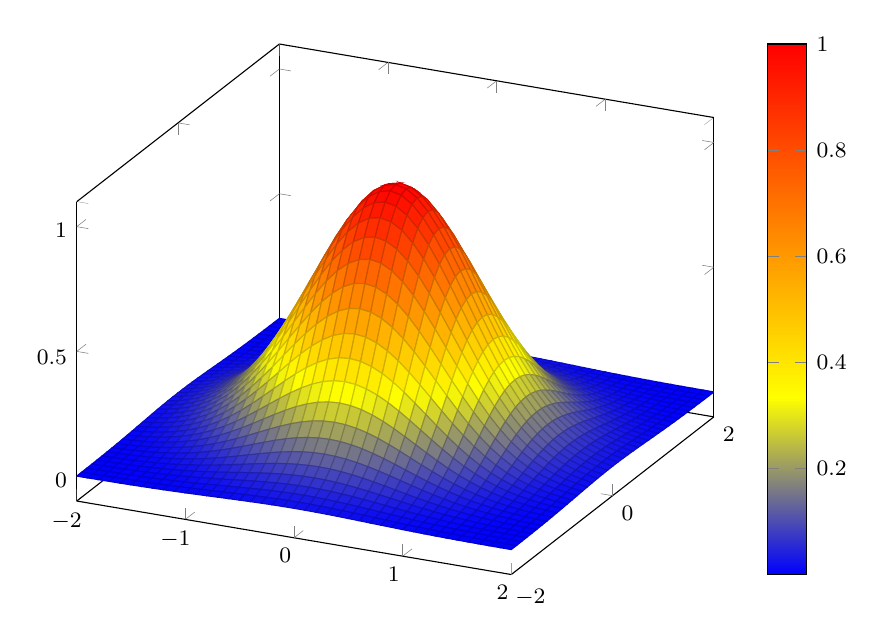
\begin{tikzpicture} 
\begin{axis}[
   colorbar,
   colorbar style={
     font=\footnotesize
   },
   width=0.45\paperwidth,
   font=\footnotesize,
]
  \addplot3[surf,samples=41,domain=-2:2] {exp(-x^2-y^2)};
\end{axis}
\end{tikzpicture}
\end{figure}
\end{frame}


\begin{frame}[fragile]{Gory details...}
De theme package bestaat uit
\begin{itemize}
\item \texttt{beamerthemethuas.sty}
\begin{itemize}
\item Deze moet je aanroepen met \lstinline|\usetheme{thuas}|
\end{itemize}
\item \texttt{beamercolorthemethuas.sty}
\begin{itemize}
\item Hierin zijn de kleuren gedefinieerd
\end{itemize}
\item \texttt{beamerinnerthemethuas.sty}
\begin{itemize}
\item Hierin is de opmaak \emph{van} de inhoud gedefinieerd (ook de titelpagina)
\end{itemize}
\item \texttt{beamerouterthemethuas.sty}
\begin{itemize}
\item Hierin is de opmaak \emph{rond} de inhoud gedefinieerd (header, footer)
\end{itemize}
\end{itemize}
\end{frame}


\begin{frame}[fragile]{Gory details...}
Er worden drie plaatjes gebruikt
\begin{itemize}
\item Plaatje op titelpagina: \lstinline|beamerthemethuasfront.pdf|
\item Logo Nederlands: \lstinline|beamerthemethuaslogo.pdf|
\item Logo Engels: \lstinline|beamerthemethuaslogo-en.pdf|
\item \alert{TODO} Plaatjes in PGF.
\end{itemize}
\end{frame}


\begin{frame}{There Is No Largest Prime Number} 
\begin{theorem}
There is no largest prime number.
\end{theorem} 
\begin{proof}
\begin{enumerate} 
\item<1-| alert@1> Suppose $p$ were the largest prime number. 
\item<2-> Let $q$ be the product of the first $p$ numbers. 
\item<3-> Then $q+1$ is not divisible by any of them. 
\item<1-> But $q + 1$ is greater than $1$, thus divisible by some prime
number not in the first $p$ numbers.
\end{enumerate}
\end{proof}
\end{frame}

\begin{frame}[fragile]{Allerlaaste slide}
De allerlaatste slide
\begin{itemize}
\item Je kan een allerlaatste slide automatisch maken met \lstinline|\beamerthemethuasbackframe|
\item In de resulterende PDF zie je dan vier verschillende slides.
\item Bij het \textsl{afspelen} met Acrobat of een \textsl{PDF aware} presenter worden de slides automatisch na elkaar afgespeed met steeds een seconde vertraging
\end{itemize}

\end{frame}

%% Make last slide
\beamerthemethuasbackframe

%%% Test slide van Jesse
%\newdimen\efkes\efkes=12.80cm
%\makeatletter
%\begin{frame}{test slide van Jesse}
%
%%% Test if babel loaded
%\ifdefined\bbl@loaded
%\bbl@loaded
%\else
%Babel not loaded
%\fi
%
%%% translater always loaded by beamer
%\trans@languages
%
%%% 12.80cm in points
%\the\efkes
%
%\end{frame}
%\makeatother

\end{document}
